\documentclass[12pt,a4paper,twoside,fleqn,notitlepage,openany]{extarticle}

\usepackage[
papersize={210mm,297mm},% Specify the paper dimensions
layoutsize={210mm,297mm}, layouthoffset=0cm, layoutvoffset=0cm, % Specify the dimensions of the layout and it's horizontal and vertical distance from the beginning of the paper.
%showcrop, % Uncomment to see the layout boundaries
top=2.4cm, includehead, % Margin from top to top of the header
bottom=3.2cm, heightrounded, % Margin from Bottom
bindingoffset=10mm, % Binding margin
inner=21mm, outer=31mm, % The inner/outer edge of the layout (inner:outer ratio in two-side is 1:1.5)
marginparwidth=0cm, marginparsep=3mm, % Specify the border width and distance from the bottom of the body of the text. (These marginal notes are placed inside the outer margin of the layout.)
%columnsep=1cm % Adjust separation between columns in two column mode.
%showframe, % This option is for drawing a border around the textbody.
]{geometry}

\usepackage{hyperref}
\usepackage{fancyhdr}
\usepackage[perpage]{footmisc}
\usepackage{float}
\usepackage{adjustbox}
\usepackage{pdfpages}
\usepackage{parsa}
\usepackage[localise,fontsloadable]{xepersian}
\settextfont{IRZar}
\defpersianfont\ParsaHeaderFont{IRNazanin}

\fancypagestyle{plain}{\fancyhf{}\fancyfoot[OL,ER]{\thepage}\renewcommand{\headrulewidth}{0pt}}

\SepMark{-}


\begin{document}
\pagestyle{plain}
\عنوان{بسته‌ی پارسا}
\نویسنده{فرشاد رسولی \thanks{\href{https://github.com/farshadrasuli/parsa}{\lr{github.com/farshadrasuli/parsa}}}}
\تاریخ{1398/09/21 - \lr{December 12, 2019}}
\عنوان‌ساز
\begin{center}
\begin{minipage}{0.67\textwidth}
تألیف پایان‌نامه و رساله، چهارچوب از پیش تعیین شده‌ای مانند چگونگی درج سربرگ، ساخت و تکمیل فرم‌های مربوطه و تدوین عناصر مختلف دارد\@. این بسته با هدف تولید فرم‌های مورد نیاز، به منطور تسریع فرآیند تألیف پایان‌نامه و رساله توسط دانشجو-پژوهش‌گر تهیه شده‌است\@. \\
امیدوارم با استفاده از این بسته، در مدت زمان تهیه‌ی پایان‌نامه و رساله، صرفه‌جویی کافی حاصل شود و به جای صرف وقت به ویرایش پایان‌نامه، زمان بیشتری به مسائل پژوهشی اختصاص یابد\@.
\end{minipage}
\end{center}
\tableofcontents
\section*{سپاس‌گزاری}
\addcontentsline{toc}{section}{سپاس‌گزاری}
از جناب آقای \موکد{وفا کارن‌پهلو} بابت تهیه و توسعه‌ی بسته‌ی \موکد{زی‌پرشین} سپاس‌گزاری می‌کنم و برای ایشان آرزوی سلامتی و سعادت دارم\@. کار بی‌نظیر ایشان در تهیه‌ی بسته‌ی زی‌پرشین، الهام بخش تهیه‌ی بسته‌ی \موکد{پارسا} بوده‌است.

\section{شروع کار}
طبقه‌ی نوشتار \زیرنویس{\متن‌لاتین{documentclass}} را از نوع کتاب انتخاب کنید و سپس با استفاده از فرمان
\[\textrm{\lr{\texttt{$\backslash$usepackage[\textrm{<options>}]\{parsa\}}}}\]
بسته‌ی پارسا فعال می‌شود\@. برای گزینه‌های این بسته، \متن‌لاتین{[\emph{<options>}]}، قسمت (\رجوع{ParsaInf}) را ببینید.\\
اکنون بسته‌ی \XePersian ~را فعال کنید\@.
\[ \textrm{ \lr{ \texttt{$\backslash$usepackage\{xepersian\}} } } \]
قلم اصلی متن را با فرمان
\[ \textrm{ \lr{ \texttt{$\backslash$settextfont\{\textrm{<font>}\} } } } \]
و قلم سربرگ را با فرمان
\[ \textrm{ \lr{ \texttt{$\backslash$defpersianfont$\backslash$ParsaHeaderFont\{\textrm{<font>}\} } } } \]
تعیین کنید\@. توصیه می‌شود برای قلم اصلی، از قلم زر \زیرنویس{توسعه‌دهندگان مختلف، نسخه‌های متفاوتی از قلم زر با نام‌های \متن‌لاتین{B Zar}،\متن‌لاتین{XB Zar} و \متن‌لاتین{IRZar} ~منتشر کرده‌اند که استفاده از \متن‌لاتین{IRZar} ~توصیه می‌شود.} و برای قلم سربرگ، از قلم نازنین \زیرنویس{از بین نسخه‌های متفاوت قلم نازنین با نام‌های \متن‌لاتین{B Nazanin}، \متن‌لاتین{XB Nazanin} و \متن‌لاتین{IRNazanin} ~استفاده از \متن‌لاتین{IRNazanin} ~توصیه می‌شود.} استفاده کنید\@.

\section{ورود اطلاعات}
برای وارد کردن اطلاعات پایان‌نامه (یا رساله)، فرمان مد نظر خود را، مطابق دستورات شرح داده‌شده، در قسمت سرآغاز \زیرنویس{\متن‌لاتین{preamble}}~وارد کنید.
\subsection{اطلاعات مؤسسه}
نام مؤسسه‌ی محل تحصیل خود را با فرمان
\[ \textrm{ \lr{ \texttt{$\backslash$Institute\{\textrm{<persian>}\}\{\textrm{<latin>}\}} } } \]
وارد کنید. دقت شود که آرگومان اول، \{\emph{<persian>}\}، برای ورود اطلاعات به زبان پارسی و آرگومان دوم، \{\emph{<latin>}\}، برای ورود اطلاعات به لاتین درنظر گرفته شده است. این اصل برای تمام فرمان‌های این بسته که دو آرگومان دارند رعایت شده است\@. به همین صورت، برای سایر اطلاعات از فرمان‌ها به شرح زیر استفاده کنید\@. \\
نشان مؤسسه:
\[ \textrm{ \lr{ \texttt{$\backslash$InstituteLogo\{\textrm{<Iranian logo>}\}\{\textrm{<International logo>}\}[\textrm{<width>}][\textrm{<height>}]} } } \]
با آرگومان‌های اختیاری، پهنا و بلندای نشان مؤسسه را، در صفحه‌ی عنوان تنظیم کنید. مقدار پیش‌فرض ۳۰×۳۰ میلی‌متر است\@. \\
نام دانش‌کده یا پژوهش‌کده:
\[ \textrm{ \lr{ \texttt{$\backslash$Faculty\{\textrm{<persian>}\}\{\textrm{<latin>}\}} } } \]
نام گروه:
\[ \textrm{ \lr{ \texttt{$\backslash$Department\{\textrm{<persian>}\}\{\textrm{<latin>}\}} } } \]
\subsection{اطلاعات نگارنده}
برای وارد کردن اطلاعات نگارنده، از فرمان‌های زیر استفاده کنید\@. چنان‌چه قصد دارید که یکی از دو آرگومان فرمانی را خالی بگذارید، کافی‌است از نشانه‌ی مد ($\sim$) استفاده کنید\@. \\
نام کامل نگارنده‌ی اثر:
\[ \textrm{ \lr{ \texttt{$\backslash$StudentName\{\textrm{<persian>}\}\{\textrm{<latin>}\}} } } \]
رشته‌ی تحصیلی:
\[ \textrm{ \lr{ \texttt{$\backslash$StudentMajor\{\textrm{<persian>}\}\{\textrm{<latin>}\}} } } \]
گرایش تحصیلی:
\[ \textrm{ \lr{ \texttt{$\backslash$StudentMinor\{\textrm{<persian>}\}\{\textrm{<latin>}\}} } } \]
مقطع تحصیلی:
\[ \textrm{ \lr{ \texttt{$\backslash$StudentDegree\{\textrm{<persian>}\}\{\textrm{<latin>}\}} } } \]
شماره ملی:
\[ \textrm{ \lr{ \texttt{$\backslash$StudentID\{\textrm{<national ID number>}\}} } } \]
شماره دانشجویی:
\[ \textrm{ \lr{ \texttt{$\backslash$StudentNumber\{\textrm{<Student Number>}\}} } } \]
رایانامه:
\[ \textrm{ \lr{ \texttt{$\backslash$StudentEMAIL\{\textrm{<sample@site.com>}\}} } } \]
\subsection{اطلاعات سند} \label{ParsaInf}
باید نوع سندی که قصد تهیه‌‌ی آن را دارید، از آن جهت که پایان‌نامه است یا رساله، مشخص کنید\@. هنگام فراخوانی بسته‌ی پارسا، امکان استفاده از گزینه‌ی \متن‌لاتین{\متن‌تایپ{thesis}} ~یا \متن‌لاتین{\متن‌تایپ{dissertation}} ~وجود دارد که گزینه‌ی \متن‌لاتین{\متن‌تایپ{thesis}} ~نوع سند را پایان‌نامه و گزینه‌ی \متن‌لاتین{\متن‌تایپ{dissertation}} ~نوع سند را رساله تعیین می‌کند. چنان‌چه از این گزینه‌ها استفاده نکردید، می‌توانید با فرمان
\[ \textrm{ \lr{ \texttt{$\backslash$ParsaTarget\{\textrm{<persian>}\}\{\textrm{<latin>}\}} } } \]
نوع سند خود را مشخص کنید\@. برای سایر اطلاعات سند، از فرمان‌های زیر استفاده کنید\@. \\
عنوان سند:
\[ \textrm{ \lr{ \texttt{$\backslash$ParsaTitle\{\textrm{<persian>}\}\{\textrm{<latin>}\}} } } \]
تاریخ تدوین که در صفحه‌ی عنوان درج می‌شود (به صورت ماه و سال وارد شود):
\[ \textrm{ \lr{ \texttt{$\backslash$ParsaCompilationDate\{\textrm{<persian date>}\}\{\textrm{<International date>}\}} } } \]
تاریخ دقیق دفاع از پایان‌نامه یا رساله:
\[ \textrm{ \lr{ \texttt{$\backslash$ParsaExamDate\{\textrm{<persian date>}\}\{\textrm{<International date>}\}} } } \]
\subsection{اطلاعات استاد راهنما} \label{SupInf}
اطلاعات استاد راهنما را با فرمان‌های زیر وارد کنید\@. \\
نام کامل استاد راهنما:
\[ \textrm{ \lr{ \texttt{$\backslash$SupervisorName\{\textrm{<persian>}\}\{\textrm{<latin>}\}} } } \]
سمت یا مرتبه‌ی علمی:
\[ \textrm{ \lr{ \texttt{$\backslash$SupervisorTitle\{\textrm{<persian>}\}\{\textrm{<latin>}\}} } } \]
وابستگی سازمانی:
\[ \textrm{ \lr{ \texttt{$\backslash$SupervisorAffiliation\{\textrm{<persian>}\}\{\textrm{<latin>}\}} } } \]
شماره ملی:
\[ \textrm{ \lr{ \texttt{$\backslash$SupervisorID\{\textrm{<national ID number>}\}} } } \]
رایانامه:
\[ \textrm{ \lr{ \texttt{$\backslash$SupervisorEMAIL\{\textrm{<sample@site.com>}\}} } } \]
\subsection{اطلاعات استاد راهنمای دوم}
همانند استاد راهنما، قسمت (\رجوع{SupInf})، اطلاعات استاد راهنمای دوم را -در صورت وجود- با فرمان‌های زیر وارد کنید\@. روند ورود اطلاعات سایر اعضای کمیته‌ی دفاع، مانند استادان مشاور، استادان داور و نماینده‌ی تحصیلات تکمیلی نیز به همین صورت می‌باشد\@. \\
نام کامل استاد راهنمای دوم:
\[ \textrm{ \lr{ \texttt{$\backslash$SecondSupervisorName\{\textrm{<persian>}\}\{\textrm{<latin>}\}} } } \]
سمت یا مرتبه‌ی علمی:
\[ \textrm{ \lr{ \texttt{$\backslash$SecondSupervisorTitle\{\textrm{<persian>}\}\{\textrm{<latin>}\}} } } \]
وابستگی سازمانی:
\[ \textrm{ \lr{ \texttt{$\backslash$SecondSupervisorAffiliation\{\textrm{<persian>}\}\{\textrm{<latin>}\}} } } \]
شماره ملی:
\[ \textrm{ \lr{ \texttt{$\backslash$SecondSupervisorID\{\textrm{<national ID number>}\}} } } \]
رایانامه:
\[ \textrm{ \lr{ \texttt{$\backslash$SecondSupervisorEMAIL\{\textrm{<sample@site.com>}\}} } } \]
\subsection{اطلاعات استاد مشاور}
اطلاعات استاد مشاور را -در صورت وجود- با فرمان‌های زیر وارد کنید\@. \\
نام کامل استاد مشاور:
\[ \textrm{ \lr{ \texttt{$\backslash$CosupervisorName\{\textrm{<persian>}\}\{\textrm{<latin>}\}} } } \]
سمت یا مرتبه‌ی علمی:
\[ \textrm{ \lr{ \texttt{$\backslash$CosupervisorTitle\{\textrm{<persian>}\}\{\textrm{<latin>}\}} } } \]
وابستگی سازمانی:
\[ \textrm{ \lr{ \texttt{$\backslash$CosupervisorAffiliation\{\textrm{<persian>}\}\{\textrm{<latin>}\}} } } \]
شماره ملی:
\[ \textrm{ \lr{ \texttt{$\backslash$CosupervisorID\{\textrm{<national ID number>}\}} } } \]
رایانامه:
\[ \textrm{ \lr{ \texttt{$\backslash$CosupervisorEMAIL\{\textrm{<sample@site.com>}\}} } } \]
\subsection{اطلاعات استاد مشاور دوم}
اطلاعات استاد مشاور دوم را -در صورت وجود- با فرمان‌های زیر وارد کنید\@. \\
نام کامل استاد مشاور دوم:
\[ \textrm{ \lr{ \texttt{$\backslash$SecondCosupervisorName\{\textrm{<persian>}\}\{\textrm{<latin>}\}} } } \]
سمت یا مرتبه‌ی علمی:
\[ \textrm{ \lr{ \texttt{$\backslash$SecondCosupervisorTitle\{\textrm{<persian>}\}\{\textrm{<latin>}\}} } } \]
وابستگی سازمانی:
\[ \textrm{ \lr{ \texttt{$\backslash$SecondCosupervisorAffiliation\{\textrm{<persian>}\}\{\textrm{<latin>}\}} } } \]
شماره ملی:
\[ \textrm{ \lr{ \texttt{$\backslash$SecondCosupervisorID\{\textrm{<national ID number>}\}} } } \]
رایانامه:
\[ \textrm{ \lr{ \texttt{$\backslash$SecondCosupervisorEMAIL\{\textrm{<sample@site.com>}\}} } } \]
\subsection{اطلاعات استاد داور اول}
اطلاعات استاد داور اول را با فرمان‌های زیر وارد کنید\@. \\
نام کامل استاد داور اول:
\[ \textrm{ \lr{ \texttt{$\backslash$FirstExaminerName\{\textrm{<persian>}\}\{\textrm{<latin>}\}} } } \]
سمت یا مرتبه‌ی علمی:
\[ \textrm{ \lr{ \texttt{$\backslash$FirstExaminerTitle\{\textrm{<persian>}\}\{\textrm{<latin>}\}} } } \]
وابستگی سازمانی:
\[ \textrm{ \lr{ \texttt{$\backslash$FirstExaminerAffiliation\{\textrm{<persian>}\}\{\textrm{<latin>}\}} } } \]
شماره ملی:
\[ \textrm{ \lr{ \texttt{$\backslash$FirstExaminerID\{\textrm{<national ID number>}\}} } } \]
رایانامه:
\[ \textrm{ \lr{ \texttt{$\backslash$FirstExaminerEMAIL\{\textrm{<sample@site.com>}\}} } } \]
\subsection{اطلاعات استاد داور دوم}
اطلاعات استاد داور دوم را -در صورت وجود- با فرمان‌های زیر وارد کنید\@. \\
نام کامل استاد داور دوم:
\[ \textrm{ \lr{ \texttt{$\backslash$SecondExaminerName\{\textrm{<persian>}\}\{\textrm{<latin>}\}} } } \]
سمت یا مرتبه‌ی علمی:
\[ \textrm{ \lr{ \texttt{$\backslash$SecondExaminerTitle\{\textrm{<persian>}\}\{\textrm{<latin>}\}} } } \]
وابستگی سازمانی:
\[ \textrm{ \lr{ \texttt{$\backslash$SecondExaminerAffiliation\{\textrm{<persian>}\}\{\textrm{<latin>}\}} } } \]
شماره ملی:
\[ \textrm{ \lr{ \texttt{$\backslash$SecondExaminerID\{\textrm{<national ID number>}\}} } } \]
رایانامه:
\[ \textrm{ \lr{ \texttt{$\backslash$SecondExaminerEMAIL\{\textrm{<sample@site.com>}\}} } } \]
\subsection{اطلاعات استاد داور سوم}
اطلاعات استاد داور سوم را -در صورت وجود- با فرمان‌های زیر وارد کنید\@. \\
نام کامل استاد داور سوم:
\[ \textrm{ \lr{ \texttt{$\backslash$ThirdExaminerName\{\textrm{<persian>}\}\{\textrm{<latin>}\}} } } \]
سمت یا مرتبه‌ی علمی:
\[ \textrm{ \lr{ \texttt{$\backslash$ThirdExaminerTitle\{\textrm{<persian>}\}\{\textrm{<latin>}\}} } } \]
وابستگی سازمانی:
\[ \textrm{ \lr{ \texttt{$\backslash$ThirdExaminerAffiliation\{\textrm{<persian>}\}\{\textrm{<latin>}\}} } } \]
شماره ملی:
\[ \textrm{ \lr{ \texttt{$\backslash$ThirdExaminerID\{\textrm{<national ID number>}\}} } } \]
رایانامه:
\[ \textrm{ \lr{ \texttt{$\backslash$ThirdExaminerEMAIL\{\textrm{<sample@site.com>}\}} } } \]
\subsection{اطلاعات نماینده‌ی تحصیلات تکمیلی}
اطلاعات نماینده‌ی تحصیلات تکمیلی را با فرمان‌های زیر وارد کنید\@. \\
نام کامل نماینده‌ی تحصیلات تکمیلی:
\[ \textrm{ \lr{ \texttt{$\backslash$RepresentativeName\{\textrm{<persian>}\}\{\textrm{<latin>}\}} } } \]
شماره ملی:
\[ \textrm{ \lr{ \texttt{$\backslash$RepresentativeID\{\textrm{<national ID number>}\}} } } \]
رایانامه:
\[ \textrm{ \lr{ \texttt{$\backslash$RepresentativeEMAIL\{\textrm{<sample@site.com>}\}} } } \]
\section{ساخت فرم‌ها}
پس از تکمیل اطلاعت لازم، با استفاده از فرمان‌های گفته‌شده، کار اصلی بسته‌ی پارسا آغاز می‌گردد\@. برای ساخت فرم‌های مدنظر، از دستورات زیر استفاده کنید.\\

\begin{table}[H] \adjustbox{pagecenter}{
\begin{tabular}{lr}
\lr{\texttt{$\backslash$titlepageParsi}}                    & صفحه‌ی عنوان به فارسی       \\
\lr{\texttt{$\backslash$ParsaPicture}}                      & عکس سرآغاز                  \\
\lr{\texttt{$\backslash$ParsaCredit}}                       & اصالت و مالکیت اثر          \\
\lr{\texttt{$\backslash$ExaminationReportPa}}               & صورت جلسه‌ی دفاع به فارسی   \\
\lr{\texttt{$\backslash$ParsaCopyleft}}                     & مجوز بهره‌برداری            \\
\lr{\texttt{$\backslash$ParsaDedicate\{\rl{تقدیم به...}\}}} & تقدیم                       \\
\lr{\texttt{$\backslash$ExaminationReportLa}}               & صورت جلسه‌ی دفاع به انگلیسی \\
\lr{\texttt{$\backslash$titlepageLatin}}                    & صفحه عنوان به انگلیسی      
\end{tabular} }
\end{table}

توجه کنید که فقط فرمان تقدیم، \textrm{\lr{\texttt{$\backslash$ParsaDedicate}}}~، به آرگومان نیاز دارد\@. متن تقدیم خود را در آرگومان این فرمان بنویسید\@. \بند
\پاراگراف{}برای نوشتن چکیده‌ی پایان‌نامه یا رساله، به زبان فارسی از محیط \متن‌لاتین{\متن‌تایپ{ParsaAbstractParsi}}~، و برای چکیده به لاتین از محیط \متن‌لاتین{\متن‌تایپ{ParsaAbstractLatin}} استفاده کنید\@. \\
\begin{latin}
\begin{minipage}{0.48\textwidth}
\begin{verbatim}
\begin{ParsaAbstractParsi}

\end{ParsaAbstractParsi}
\end{verbatim}
\end{minipage}
\begin{minipage}{0.48\textwidth}
\begin{verbatim}
\begin{ParsaAbstractParsi}

\end{ParsaAbstractParsi}
\end{verbatim}
\end{minipage}
\end{latin}
~\بند
برای نوشتن متن سپاس‌گزاری از محیط \متن‌لاتین{\متن‌تایپ{ParsaAcknowledgment}} ~استفاده کنید.\\
\begin{latin}
\begin{verbatim}
\begin{ParsaAcknowledgment}

\end{ParsaAcknowledgment}
\end{verbatim}
\end{latin}

\section{کدهای آماده}
کدهای زیر برای استفاده در \LaTeX ~برای شما آماده شده‌است. برای استفاده از هر کد، کافی‌است علامت درصد ابتدای هرخط را حذف کنید.
\begin{latin}
\begin{verbatim}
\documentclass[a4paper,12pt,twoside]{book}

\usepackage{parsa}
\usepackage[fontsloadable]{xepersian}
\settextfont{} 
\defpersianfont\ParsaHeaderFont{} 



%------------------------------------------------------------------
%	THESIS/DISSERTATION INFORMATION STARTS FROM HERE:
%

% --- Institute's Information
%\InstituteLogo{}{}[][] 
%\Institute{}{}
%\Faculty{}{}
%\Department{}{} 

% --- Student's Information
%\StudentName{}{} 
%\StudentMajor{}{}
%\StudentMinor{}{}
%\StudentDegree{}{}
%\StudentID{}
%\StudentNumber{}
%StudentEMAIL{}

% --- Thesis/Dissertation's Information
%\ParsaTitle{}{} % {<persian>}{<latin>}
%\ParsaCompilationDate{}{} % {<persian date>}{<latin date>}
%\ParsaExamDate{}{} % {<persian date>}{<latin date>}

% --- Members of The Committee's Informtion
%\SupervisorName{}{} 
%\SupervisorTitle{}{}
%\SupervisorAffiliation{}{}
%\SupervisorID{}
%\SupervisorEMAIL{}

%\SecondSupervisorName{}{}
%\SecondSupervisorTitle{}{}
%\SecondSupervisorAffiliation{}{}
%\SecondSupervisorID{}
%\SecondSupervisorEMAIL{}

%\CosupervisorName{}{}
%\CosupervisorTitle{}{}
%\CosupervisorAffiliation{}{}
%\CosupervisorID{}
%\CosupervisorEMAIL{}

%\SecondCosupervisorName{}{}
%\SecondCosupervisorTitle{}{}
%\SecondCosupervisorAffiliation{}{}
%\SecondCosupervisorID{}
%\SecondCosupervisorEMAIL{}

%\FirstExaminerName{}{}
%\FirstExaminerTitle{}{}
%\FirstExaminerAffiliation{}{}
%\FirstExaminerID{}
%\FirstExaminerEMAIL{}

%\SecondExaminerName{}{}
%\SecondExaminerTitle{}{}
%\SecondExaminerAffiliation{}{}
%\SecondExaminerID{}
%\SecondExaminerEMAIL{}



%\ThirdExaminerName{}{}
%\ThirdExaminerTitle{}{}
%\ThirdExaminerAffiliation{}{}
%\ThirdExaminerID{}
%\ThirdExaminerEMAIL{}

%\RepresentativeName{}{}
%\RepresentativeID{}
%\RepresentativeEMAIL{}

%
%	THESIS/DISSERTATION INFORMATION ENDED.
%------------------------------------------------------------------

\begin{document}

\titlepageParsi
\newpage

%-----------------------------------------------
%	PERSIAN ABSTRACT STARTS FROM HERE:
%
\begin{ParsaAbstractParsi}

\end{ParsaAbstractParsi}
%
%	PERSIAN ABSTRACT ENDED.
%-----------------------------------------------

\ParsaPicture{}

\ParsaCredit
\newpage

\ExaminationReportPa
\newpage

\ParsaCopyleft
\newpage

\ParsaDedicate{}




%--------------------------------------------------
%	ACKNOWLEDGMENT STARTS FROM HERE:
%
\begin{ParsaAcknowledgment}

\end{ParsaAcknowledgment}
%
%	ACKNOWLEDGEMENT ENDED.
%--------------------------------------------------
\newpage

%--------------------------------------------------
%	CV STARTS FROM HERE:
%
\begin{ParsaCV}

\end{ParsaCV}
%
%	CV ENDED.
%--------------------------------------------------


\ExaminationReportLa
\newpage

%-----------------------------------------------
%	LATIN ABSTRACT STARTS FROM HERE:
%
\begin{ParsaAbstractLatin}

\end{ParsaAbstractLatin}
%
%	LATIN ABSTRACT ENDED.
%-----------------------------------------------

\titlepageLatin

\end{document}
\end{verbatim}
\end{latin}

\section{نمونه پایان‌نامه}
در صفحات بعدی، نمونه‌ای از پایان نامه‌ی انجام‌شده به کمک بسته‌ی پارسا قرار گرفته‌است. \\
\cleardoublepage

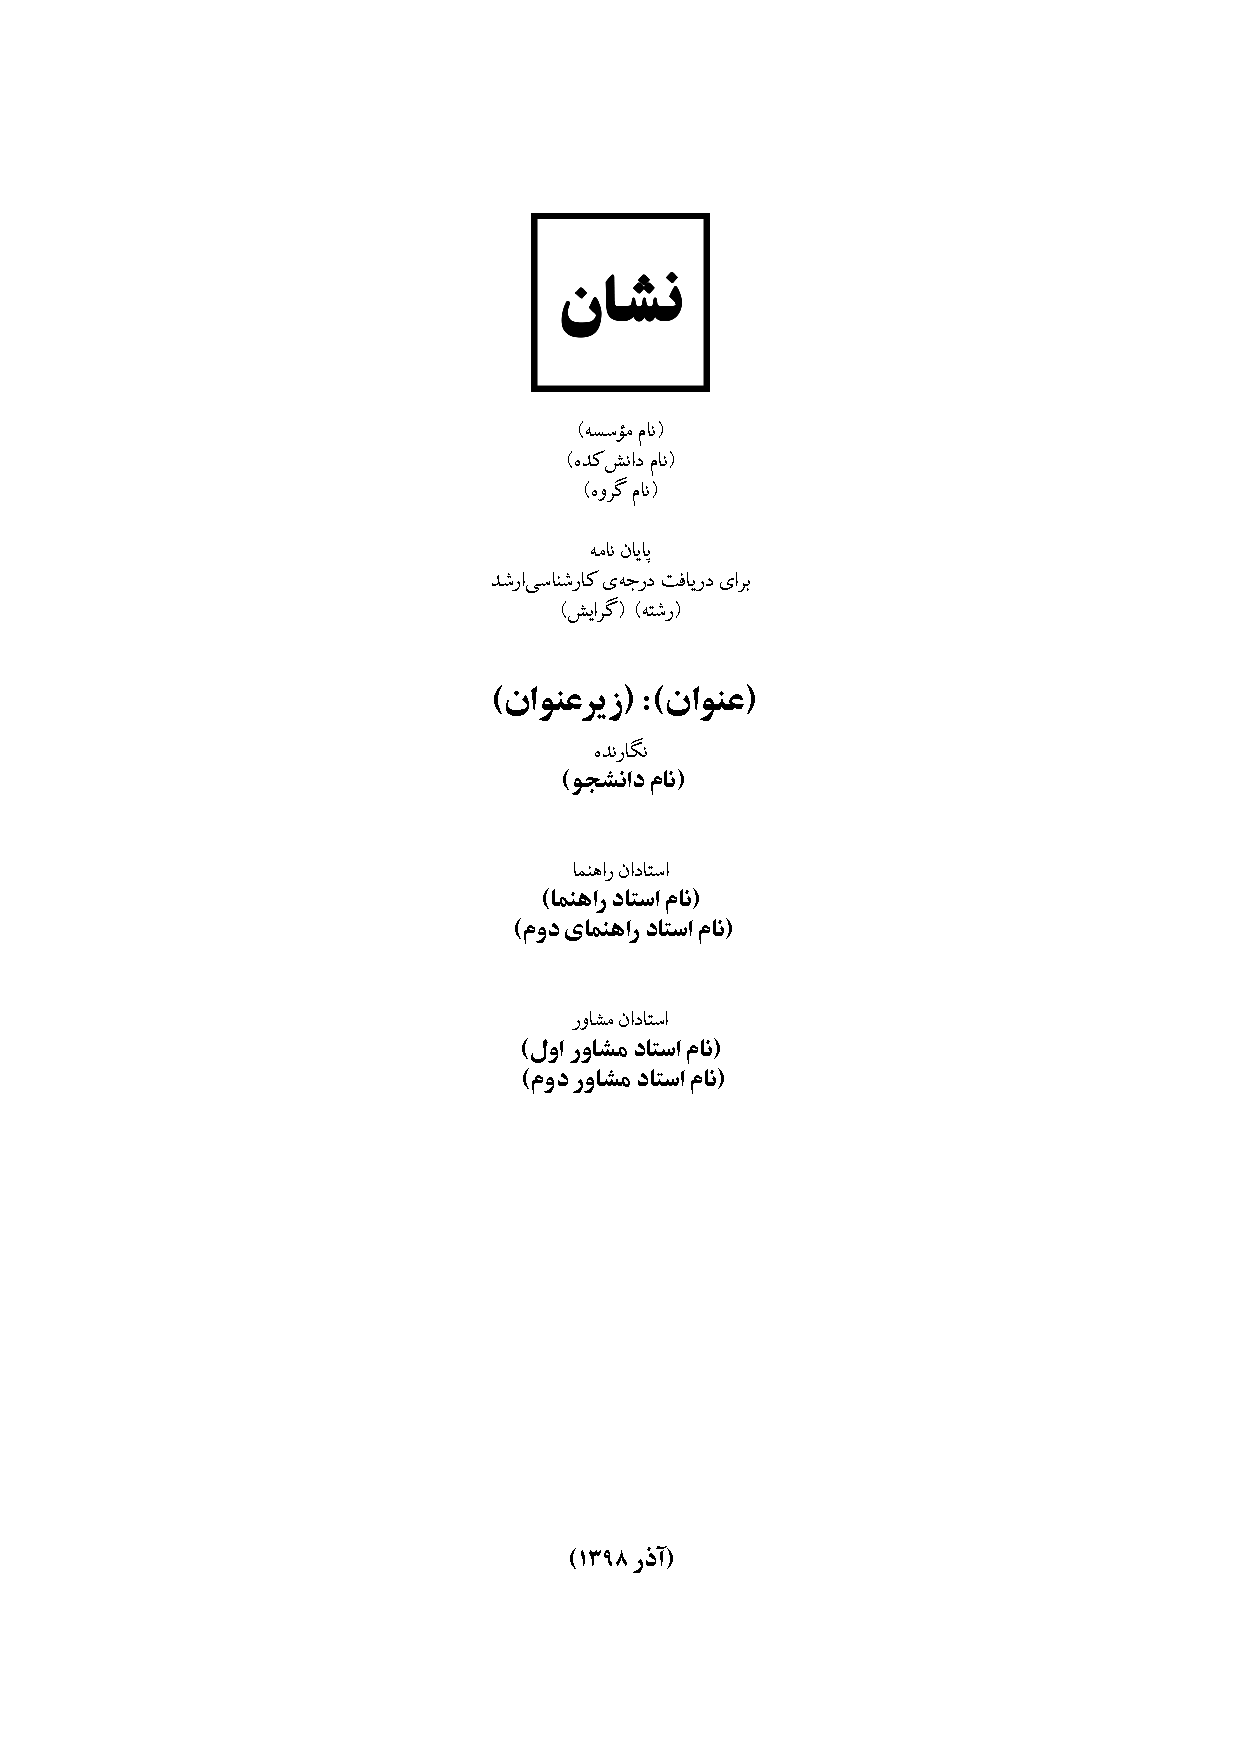
\includepdf[page=-]{minimaltemplate}
\end{document}
